%!TEX TS-program = xelatex
%!TEX encoding = UTF-8 Unicode
%!TeX spellcheck = it_IT

\documentclass{Dissertate}

%----------------------------------------------------------------------------------------
%	PACKAGES AND SETTINGS
%----------------------------------------------------------------------------------------

\usepackage[italian]{babel}
\usepackage{graphicx}	% graphics
% \usepackage[utf8x]{inputenc} % codec
% \usepackage{amsmath}	% formulas
\usepackage{hyperref}	% hyperlinks
\usepackage{algorithm}	% pseudocode for algorithms
\usepackage[noend]{algpseudocode} % same as above
\usepackage{../utils/mymacros} % macros
\usepackage{xcolor} % for colors (like in codes)
\usepackage{colortbl} %
\usepackage{listings}	% code
\definecolor{codegreen}{rgb}{0,0.6,0}
\definecolor{codegray}{rgb}{0.5,0.5,0.5}
\definecolor{backcolor}{rgb}{0.98,0.98,0.98}
\definecolor{RoyalBlue}{rgb}{0.25, 0.41, 0.88}
\definecolor{Peach}{rgb}{1.0, 0.9, 0.71}
\definecolor{SeaGreen}{rgb}{0.18, 0.55, 0.34}
\definecolor{gray}{rgb}{0.4,0.4,0.4}
\definecolor{darkblue}{rgb}{0.0,0.0,0.6}
\definecolor{cyan}{rgb}{0.0,0.6,0.6}

\renewcommand{\lstlistingname}{Codice}% Listing -> codice
\renewcommand{\lstlistlistingname}{Frammenti di codice}% List of Listings -> Frammenti di codice

\lstdefinestyle{mystyle}{
    backgroundcolor=\color{backcolor},
    commentstyle=\color{Peach}\ttfamily,
    keywordstyle=\color{RoyalBlue},
    numberstyle=\tiny\color{codegray},
    stringstyle=\color{SeaGreen}\ttfamily,
    basicstyle=\footnotesize\ttfamily,
    breakatwhitespace=false,
    breaklines=true,
    captionpos=b,
    keepspaces=true,
    numbers=left,
    numbersep=5pt,
    showspaces=false,
    showstringspaces=false,
    showtabs=false,
    tabsize=2,
    frame=trbl, % draw a frame at the top, right, left and bottom of the listing
	frameround=ftff, % angolo in basso a destro curvo
	framesep=4pt, % quarter circle size of the round corners,
	inputencoding=utf8x,
    %extendedchars=true,
    %literate={á}{{\'a}}1 {à}{{\`a}}1 {é}{{\'e}}1 {è}{{\`e}}1 {ù}{{\`u}}1 {ò}{{\`o}}1 {ì}{{\`i}}1,
    belowskip=1em,
    aboveskip=1em,
}
\lstset{style=mystyle}

\lstdefinelanguage{JavaScript}
{
  % list of keywords
  morekeywords={ true, false, catch, function, break,	new, class, extends, var, require, switch, return, import, if, while, for, this, View, Text, StyleSheet},
  sensitive=false, % keywords are not case-sensitive
  morecomment=[l]{//}, % l is for line comment
  morecomment=[s]{/*}{*/}, % s is for start and end delimiter
  morestring=[b]' % defines that strings are enclosed in double quotes
}

\lstdefinelanguage{Properties}
{
	% list of keywords
	morekeywords={ true, false, catch, function, break,	new, class, extends, var, require, switch, return, import, if, while, for, this, View, Text, StyleSheet},
	sensitive=false, % keywords are not case-sensitive
	morecomment=[l]{\#}, % l is for line comment
	morecomment=[s]{/*}{*/}, % s is for start and end delimiter
	morestring=[b]' % defines that strings are enclosed in double quotes
}

\lstdefinelanguage{JSON}
{
  % list of keywords
  morekeywords={string, boolean, int, Array, Node, Asset, AssetDetail, Filter, FilterItem},
  sensitive=false, % keywords are not case-sensitive
  morecomment=[l]{//}, % l is for line comment
  morecomment=[s]{/*}{*/}, % s is for start and end delimiter
  morestring=[b] % defines that strings are enclosed in double quotes
}

\colorlet{punct}{red!60!black}
\definecolor{background}{HTML}{EEEEEE}
\definecolor{delim}{RGB}{20,105,176}
\colorlet{numb}{magenta!60!black}

\lstdefinelanguage{json}{
    basicstyle=\normalfont\ttfamily,
    numbers=left,
    numberstyle=\scriptsize,
    stepnumber=1,
    numbersep=8pt,
    showstringspaces=false,
    breaklines=true,
    frame=lines,
    backgroundcolor=\color{background},
    literate=
     *{0}{{{\color{numb}0}}}{1}
      {1}{{{\color{numb}1}}}{1}
      {2}{{{\color{numb}2}}}{1}
      {3}{{{\color{numb}3}}}{1}
      {4}{{{\color{numb}4}}}{1}
      {5}{{{\color{numb}5}}}{1}
      {6}{{{\color{numb}6}}}{1}
      {7}{{{\color{numb}7}}}{1}
      {8}{{{\color{numb}8}}}{1}
      {9}{{{\color{numb}9}}}{1}
      {:}{{{\color{punct}{:}}}}{1}
      {,}{{{\color{punct}{,}}}}{1}
      {\{}{{{\color{delim}{\{}}}}{1}
      {\}}{{{\color{delim}{\}}}}}{1}
      {[}{{{\color{delim}{[}}}}{1}
      {]}{{{\color{delim}{]}}}}{1},
}

\lstdefinelanguage{URM}
{
	% list of keywords
	morekeywords={ S, J, T, Z, I},
	sensitive=false, % keywords are not case-sensitive
	morecomment=[l]{//}, % l is for line comment
	morecomment=[s]{/*}{*/}, % s is for start and end delimiter
	morestring=[b]' % defines that strings are enclosed in double quotes
}

\lstdefinelanguage{RDFA}{
	language=html,
	sensitive=true,
	alsoletter={<>=-},
	ndkeywords={
		% General
		=,
		% HTML attributes
		charset=, id=, width=, height=, property=, about=, rel=, rev=, prefix=, vocab=, content=, datatype=
	},
	morecomment=[s]{<!--}{-->},
	tag=[s]
}

\lstdefinestyle{BashStyle}{
  language=bash,
  basicstyle=\small\sffamily,
  numbers=left,
  numberstyle=\tiny,
  numbersep=3pt,
  frame=tb,
  columns=fullflexible,
  backgroundcolor=\color{yellow!20},
  linewidth=0.9\linewidth,
  xleftmargin=0.1\linewidth,
  framexleftmargin=0.2em}

\lstdefinestyle{myJSON}{
    language=json,
    basicstyle=\tiny,
	numbers=none}


% \lstdefinestyle{makefile}{
%   otherkeywords={.SUFFIXES},
%   alsoletter={:},
%   morekeywords=[1]{SUFFIX, CPP_},
%   morekeywords=[2]{vasp:,makeparam:,zgemmtest:,dgemmtest:,ffttest:,kpoints:,clean:},
%   style=global,%
%   morecomment=[l][commentstyle]{\#},%
%   emphstyle={\color{vimvert}},%
%   moredelim=[s][\color{vimvert}]{\$(}{)}%
%   }

\lstdefinelanguage{XML}
{
  morestring=[b]",
  morestring=[s]{>}{<},
  morecomment=[s]{<?}{?>},
  stringstyle=\color{black},
  identifierstyle=\color{darkblue},
  keywordstyle=\color{cyan},
  morekeywords={xmlns,version,type}% list your attributes here
}
 %
\lccode`~=0 %
\usepackage{multirow}		% merge cell vertically in tabels
\usepackage[fixlanguage]{babelbib}	% bibliography language
\selectbiblanguage{italian}

\graphicspath{{figures/}}	% image path

\begin{document}

%----------------------------------------------------------------------------------------
%	TITLE PAGE AND HEADERS
%----------------------------------------------------------------------------------------

% the front matter
%!TEX TS-program = xelatex
%!TEX encoding = UTF-8 Unicode
%!TeX spellcheck = it_IT
%!TEX root = ../tesi.tex

% Some details about the dissertation.
\title{Ombreggiatura in NS-3}
\author{Marco Romanelli}

%If you have one advisor
\advisor{Claudio Enrico Palazzi}

%If you are coadvised
% \coadvisorOne{Delightful Researcher}
% \coadvisorOneUniversity{Università Blabla}

\mastername{Laurea Magistrale in Informatica}

\academicyear{2016-2017}

% \maketitle
% \copyrightpage
\frontmatter
\setstretch{\dnormalspacing}
% \tableofcontents
% %\authorlist
% \listoffigures
% \dedicationpage
% \acknowledgments

\doublespacing

%----------------------------------------------------------------------------------------
%	BODY
%----------------------------------------------------------------------------------------
\setcounter{chapter}{0}  % start chapter numbering at 1
%!TEX TS-program = xelatex
%!TEX encoding = UTF-8 Unicode
%!TeX spellcheck = it_IT
%!TEX root = ../tesi.tex

\chapter{Introduzione}\label{chap:introduction}
% \section{Contesto}\label{sec:contesto}
% scaletta:
% - introdurre le vanet
% - importanza della propagazione/protocolli broadcast
% - importanza delle simulazioni
% - importanza di simulazioni veritiere
% - (~) modelli per rendere migliori le simulazioni
% - importanza degli ostacoli
% - modellazione di ambiente 3d
% - struttura documenti tesi
I progressi tecnologici dell'ultimo decennio nell'hardware, nel software e nelle telecomunicazioni hanno permesso
la larga diffusione di unità computazionali all'interno degli autoveicoli. % , anche in quelli di fascia medio-bassa.
Questo ha portato a un incremento dell'interesse della ricerca scientifica in questo campo e, in particolare,
sullo studio delle reti veicolari o VANET (\textit{Vehicular Ad-hoc Networks}).

Le VANET rappresentano una famiglia delle reti Ad-hoc mobili (\textit{Mobile Ad-hoc Network}, MANET)
nelle quali i movimenti sono strutturati, i veicoli possono essere consapevoli della propria posizione nello spazio (ad esempio tramite geolocalizzazione GPS)
e spesso sono equipaggiati con attrezzatura che permette le comunicazioni inter-veicolari (es.~antenne radio).
Queste reti sono alla base di una vasta gamma di necessità, che spaziano dalla sicurezza stradale alle applicazioni multimediali,
dalla distribuzione dei dati sul traffico allo sviluppo di una rete infrastrutturale urbana.

Una caratteristica comune è la necessità di un sistema che propaghi le informazioni
con il minor ritardo possibile; per esempio un pericolo inatteso sulla careggiata potrebbe causare l'impossibilità di proseguire
lungo il percorso ed è necessario informare i veicoli che seguono.
Oppure all'interno di una trasmissione di contenuti multimediali (giochi mutiplayer, video) fra due o più veicoli
alte latenze potrebbero inficiare la fruizione dei contenuti~\cite{1580935}~\cite{PantelW02}.
Una delle soluzioni proposte si chiama Fast Broadcast: un protocollo per ridurre il tempo di propagazione
di un messaggio da una sorgente a una destinazione tramite una stima del raggio trasmissivo effettivo e
il conseguente utilizzo di questa per ridurre il numero di salti necessari al raggiungimento dell'obiettivo~\cite{Palazzi07howdo}.

La valutazione di protocolli di questo tipo su scenari urbani con migliaia di agenti risulta
problematica principalmente a causa dei costi proibitivi (oltre alle implicazioni sulla privacy)
che comporterebbe una sperimentazione nel mondo reale.
Spesso i ricercatori ricadono, quindi, sull'utilizzo di modelli simulati eventualmente integrati con risultati ottenuti
da esperimenti sul campo in ambienti ridotti e controllati.
In particolare, l'accuratezza dei modelli di propagazione e di mobilità rappresenta la chiave per una buona valutazione delle prestazioni
dei protocolli di rete veicolari~\cite{4020783}.
All'interno di scenari urbani e suburbani gli edifici ostruiscono la naturale propagazione di un segnale radio nello spazio
e, di conseguenza, al fine di eseguire simulazioni più affidabili questa ostruzione non può essere ignorata.
Una fra le diverse soluzioni proposte negli anni permette di calcolare l'attenuazione del segnale per un singolo edificio
in funzione del numero di intersezioni con le pareti esterne e la distanza interna percorsa~\cite{5720204}.
Qualche anno più tardi, il modello è stato ripreso, implementato per uno software di simulazioni
e integrato con informazioni reali sulla geometria degli edifici e sulla topologia stradale~\cite{Carpenter:2015:OMI:2756509.2756512}.
Un aspetto positivo di questo modello risiede nella sua implementazione, rilasciata
come modulo aggiuntivo per Network Simulator 3 (ns-3)~\cite{ns3Website},
ultima versione della nota famiglia di simulatori di rete, successore di ns-2
e l'unica a essere attualmente mantenuta.
ns-3 è assieme a \omnet~\cite{omnetWebsite} uno dei simulatori più diffusi
in ambito accademico e di ricerca, grazie alla loro natura \textit{open-source},
all'ambiente di configurazione delle simulazioni in \Cpp{} e a una comunità di sviluppo attiva.
Considerato questo e la presenza di una implementazione sia del modello a ostacoli
che del protocollo Fast Broadcast per ns-3 la scelta del simulatore da utilizzare
è ricaduta su quest'ultimo.

Riassumendo, risulta interessante analizzare l'impatto che l'effetto ombreggiatura derivato dalla
presenza di edifici, e ostacoli in generale, ha sulla propagazione dei messaggi e
sulle prestazioni del protocollo Fast Broadcast. % ci starebbe un e.., ma cosa mettere?
%
\paragraph{}
Il presente lavoro è strutturato come segue.
Nel capitolo successivo (Capitolo~\ref{chap:protocollo-fast-broadcast}) verrà presentato il protocollo Fast Broadcast e una proposta di estensione in due dimensioni.
Il Capitolo~\ref{chap:modello-a-ostacoli} analizzerà il modello a ostacoli, sia dal punto di vista matematico che da quello analitico inerente alla simulazione;
concluderà presentando una possibile soluzione per rendere il modello tridimensionale.
Il Capitolo~\ref{chap:applicativi} darà una veloce panoramica sui software utilizzati e il metodo utilizzato per la creazione degli scenari.
Il Capitolo~\ref{chap:simulazioni} illusterà i diversi gruppi di simulazioni effettuati e i relativi risultati ottenuti.
Infine, nel Capitolo~\ref{chap:conclusioni}
si concluderà riassumento i risultati ed evidenziando alcuni possibili sviluppi.
%
\section{Modelli di radiopropagazione}\label{sec:modelli-propagazione}
Un modello di radiopropagazione (MRP) simula gli effetti dell'attenuazione del segnale radio (segnali elettromagnetici nello spazio libero o etere, in contrasto con la propagazione guidata)
dovuta alla distanza, cammini multipli per effetto della riflessione, ombreggiatura causata dalla presenza di ostacoli.
L'utilizzo di un'idonea rappresentazione per questo tipo di ostacoli è, quindi, necessaria nel contesto di simulazioni di reti VANET in ambienti urbani
e suburbani.
Nel corso degli anni, diversi MRP sono stati proposti.
Il più semplice di questi si chiama modello a disco unitario (\textit{unit-disk model}), nel quale i veicoli possono comunicare fra loro se si trovano entro una certa soglia
di distanza, mentre non possono altrimenti~\cite{6554832}.
Un modello molto utilizzato nelle simuazioni di VANET è il modello a doppio raggio (\textit{Two-ray ground-reflection model}),
nel quale il segnale in fase di ricezione è composto da una componente in linea diretta e una seconda derivante dalla riflessione causata dal terreno~\cite{DBLP:books/daglib/0091821}.
In~\cite{Schmitz:2006:ERW:1164717.1164730} e in~\cite{Souley2005RealisticUS}, modelli più sviluppati prendono in considerazione anche le proprietà riflettenti delle superfici e degli ostacoli.

Tuttavia, un approcio diretto di questo tipo difficilmente scala al numero di nodi necessario in un classico scenario VANET e per questo motivo
spesso tali modelli si affidano a una fase di pre-elaborazione che può richiedere tempi elevati~\cite{Stepanov:2008:IMR:1293378.1293656}.
Per ovviare a questo problema, alcune proposte astraggono dalle informazioni sui singoli edifici, modellando l'ambiente urbano in modo omogeneo
così da creare un modello analitico per l'ombreggiatura~\cite{1492678}.
Questo tipo di modelli riducono il costo computazionale e generalmente si raffrontano bene con i risultati reali;
ciò nonostante, non riescono a catturare effetti a livello mesoscopico come eventuali spazi fra edifici che permetterebbero trasmissioni a corto raggio~\cite{Giordano:2010:CST:1860058.1860065}.

Sono affetti dallo stesso problema anche i modelli (puramente) probabilistici, in quanto non tengono in considerazione la geometria urbana sottostante.
Questi modellano l'effetto dell'ombraggiatura tramite distribuzione stocastiche, fra cui Rice, Rayleigh, Nakagami-m, lognormale e Weibull~\cite{6554832}~\cite{Rappaport:2001:WCP:559977}.
%
\section{Modellazione di ostacoli}\label{sec:modellazione-ostacoli}
Nelle simulazioni di alcuni scenari, come possono essere le VANET, un'accurata rappresentazione della topologia dell'ambiente è necessaria
in quanto limita non solo la mobilità dei veicoli ma interferisce anche con le trasmissioni radio~\cite{7543980}~\cite{amjad2015impact}.
L'attenuazione radio viene spesso modellata in modo deterministico basandosi principalmente sulla distanza della visuale (\textit{Line Of Sight}, LOS)
fra i veicoli, combinando eventualmente un modelli stocastico per considerare l'ombreggiatura.

Negli ultimi anni, diversi studi hanno cercato di rappresentare meglio l'effetto ombreggiatura causato dagli edifici.
In~\cite{Giordano:2010:CST:1860058.1860065} gli autori utilizzavano tecniche di geocodifica inversa (\textit{reverse geocoding}) per estrapolare
informazioni sulla topologia della rete stradale in stile Manhattan. Da qui veniva derivata la geometria degli edifici utilizzata
per differenziare i casi in cui i due veicoli comunicanti avessero la visuale libera (LOS) o meno (\textit{Non Line Of Sight}, NLOS)
e calcolare di conseguenza la potenza del segnale in ricezione.
La configurazione a griglia non è tuttavia applicabile in ogni scenario urbano, speciamente in città italiane storiche,
dove la reste stradale è molto irregolare.
In~\cite{4020783}, invece, le informazioni sugli edifici erano codificate direttamente all'interno dell'ambiente sviluppato, chiamato
EGRESS (\textit{Enviroment for Generating REalistic Scenarios for Simulations}), e permettavano di definire tre tipologie di edifici e altrettanti
percorsi per simulare la mobilità dei nodi; il modello permetteva anche di configurare, con alcuni limiti, diversi tipi di materiale dei pavimenti e dei muri degli edifici.
Questa categorizzazione non permetteva però una buona scalabilità, se si considera che in pochi kilometri quadrati di una città media
ci sono miglialia di edifici.
Gli autori di~\cite{Carpenter:2015:OMI:2756509.2756512} integravano nel noto simulatore di reti Network Simulator 3 (ns-3)~\cite{ns3Website}
un modello a ostacoli empirico precedentemente sviluppato~\cite{5720204} ed
estraevano le informazioni per la geometria degli edifici da una piattaforma gratuita
chiamata OpenStreetMap (OSM)~\cite{osmWebsite}; queste venivano successivamente elaborate da un software per la simuazione della mobilità di veicoli
e utilizzate nel simulatore, differenziando i dati sugli edifici e quelli sulla mobilità dei veicoli;
il modello di propagazione teneva conto della distanza percorsa dal segnale internamente all'ostacolo e del numero di muri esterni che questo attraversava.
La semplicità computazionale, l'assenza di pre-elaborazioni, la possibilità di integrare informazioni reali sull'ambiente
e l'integrazione con ns-3 erano alcuni dei punti a favore di questo modello.
%

%!TEX TS-program = xelatex
%!TEX encoding = UTF-8 Unicode
%!TeX spellcheck = it_IT
%!TEX root = ../tesi.tex

\chapter{Protocollo Fast Broadcast}\label{chap:protocollo-fast-broadcast}
La tecnica del Fast Broadcast~\cite{Palazzi07howdo} si compone di due fasi. La prima, chiamata ``Fase di stima'', permette a ogni veicolo di avere una stima aggiornata
del proprio raggio trasmissivo.
La seconda, invece, è detta ``Fase di inoltro'' e viene attivata nel momento in cui si rende necessario inviare un messaggio
al resto dei veicoli presenti nell'area di interesse.
%
\section{Fase di stima}\label{sec:fb-fase-di-stima}
Durante questa fase, ogni veicolo effettua una stima del suo raggio trasmissivo, sia di fronte che alle sue spalle, attraverso l'uso di messaggi \textit{Hello}.
Per ottenere una stima sempre aggiornata, il tempo è suddiviso in turni e le informazioni raccolte durante un certo turno
rimangono attive per tutto il turno successivo, per poi essere scartate.
Una breve durata dei turni permette di cogliere meglio variazioni del raggio trasmissivo mantendendo tuttavia un elevato scambio di messaggi;
gli autori suggeriscono un tempo pari a un secondo.

Le informazioni sulla stima sono rappresentate dai campi \textit{Current-turn Maximum Front Range} (CMFR) e \textit{Current-turn Maximum Back Range} (CMBR).
Il primo esprime la stima della massima distanza in avanti dalla quale un altro veicolo nell'area di interesse può ricevere messaggi che provengono dal veicolo considerato.
Il secondo, invece, stima la massima distanza all'indietro.
Questi valori sono costantemente aggiornati con i valori ricevuti nei messaggi Hello fino alla fine del turno;
dopodiché vengono salvati nei campi \textit{Latest-turn Maximum Front Range} (LMFR) e \textit{Latest-turn Maximum Back Range} (LMBR) rispettivamente.
Questo permette di combinare una stima calcolata nel tempo (con diversi messaggi Hello) con le ultime informazioni sul mezzo trasmissivo.

Nel dettaglio, la procedura di invio di un messaggio Hello prevede inizialmente che il veicolo aspetti un tempo d'attesa casuale e,
dopo aver verificato l'assenza di altre trasmissioni in corso e/o collisioni, proceda poi all'invio del messaggio contenente
la stima del raggio trasmissivo in avanti.
Vengono poi aggiunte altre informazioni utili al protocollo, come ad esempio la posizione aggiornata del veicolo.

Si fa notare che, in ogni turno, non più di un messaggio Hello viene inviato fra veicoli all'interno dell'area delimitata dal raggio trasmissivo.
In questo modo il numero totale di messaggi Hello generati rimane limitato nell'ordine di \BigO{1}.

In fase di ricezione, un veicolo determina la distanza fra lui e chi ha spedito il messaggio: se proviene da davanti sarà aggiornato il campo CMFR,
altrimenti se proviene dal retro verrà aggiornato il campo CMBR.
In ogni caso, la nuova stima sarà calcolata come il massimo fra il vecchio valore, la distanza fra i due veicoli e la stima inviata dall'altro veicolo
(e ricevuta nel messaggio di Hello).

Gli algoritmi~\ref{fig:algoritmo-invio-msg-hello} e~\ref{fig:algoritmo-ricezione-msg-hello} riassumono l'invio e la ricezione di un messaggio Hello.
%
\begin{italianalgorithm}[h]
\caption{Invio di un messaggio Hello.}\label{fig:algoritmo-invio-msg-hello}
\begin{algorithmic}[1]
	\ForEach{turno}
		\State{tempoInvio $\gets$ generaCasualmente(dimTurno)}
		\State{aspetta(tempoInvio)}
		\If{$\neg$ (RilevatomsgInoltro() $\vee$ RilevataCollisione())}
			\State{msgInoltro.portataMassima $\gets$ max(LMR, CMR)}
			\State{msgInoltro.posizione $\gets$ rilevaPosizione()}
			\State{inviaInBroadcast(msgInoltro)}
		\EndIf{}
	\EndFor{}
\end{algorithmic}
\end{italianalgorithm}
%
\begin{italianalgorithm}[h]
\caption{Ricezione di un messaggio Hello.}\label{fig:algoritmo-ricezione-msg-hello}
\begin{algorithmic}[1]
	\State{portata $\gets$ msgInoltro.portataMassima}
	\State{posizioneMittente $\gets$ helloMsg.posizione}
	\State{posizione $\gets$ rilevaPosizione()}
	\State{distanza $\gets$ calcolaDistanza(posizione, posizioneMittente)}
	\State{CMR $\gets$ max(CMR, distanza, portata)}
\end{algorithmic}
\end{italianalgorithm}
%
\section{Fase di inoltro}\label{sec:fb-fase-inoltro}
Lo scopo di questa fase consiste nel determinare il veicolo migliore per inoltrare un messaggio.
Questo viene fatto sfruttando le informazioni sulla stima del raggio trasmissivo raccolte nella fase precedente:
ogni veicolo si assegna una priorità nell'inoltro basandosi sulla distanza dal veicolo che ha trasmesso il messaggio;
la priorità cresce all'aumentare della distanza.

All'attivazione di questa fase, viene generato un messaggio di \textit{Broadcast} che dev'essere propagato lungo tutta l'area di interesse del mittente.
All'interno troviamo due campi di interesse: la posizione del veicolo e la stima del raggio trasmissivo; quest'ultima, caratteristica proprio di questo protocollo,
rappresenta quanto all'indietro ci si aspetta che arrivi il segnale prima che diventi troppo debole da non essere rilevabile.

Questo valore sarà poi sfruttato per determinare quale veicolo dovrà inoltrare il messagio in modo da minimizzare il numero di salti (\textit{hop}) e di conseguenza
ridurre il tempo di propagazione.
Nel dettaglio, quando un veicolo deve inviare o inoltrare un messaggio Broadcast calcola il valore del campo MaxRange come il massimo fra l'LMBR e il CMBR.

In fase di ricezione, un veicolo attente una quantità di tempo determinata in maniera casuale partendo dal valore di una finestra di contesa (\textit{contention window}).
Il valore di questa finestra varia fra un valore minimo (\textit{CWMin}) e un valore massimo (\textit{CWMax}), in funzione della distanza dal veicolo che ha inviato il messaggio
e la stima del raggio trasmissivo secondo la formula espressa in~\ref{eq:contention-window}.
È facile vedere come maggiore è la distanza dal mittente e minore è l'intervallo d'attesa.
\begin{gather}\label{eq:contention-window}
	\left\lfloor \left( \frac{\text{PortataMassima} - \text{Distanza}}{\text{PortataMassima}} \times (\text{CWMax} - \text{CWMin}) \right) + \text{CWmin}  \right\rfloor
\end{gather}

Se durante l'attesa viene ricevuto lo stesso messaggio proveniente dai veicoli che seguono, ciò significa che il messaggio è già stato propagato in avanti e quindi non è necessario
che il veicolo corrente lo inoltri.
Se, invece, a inviarlo è un veicolo che precede significa che il messaggio è già stato inoltrato da un altro mezzo; la procedura quindi dev'essere riavviata includendo i parametri appena ricevuti.
Nel caso in cui l'attesa finisca senza aver ricevuto nessun altro messaggio (o collisioni), il veicolo può procedere con l'inoltro includendo nei dati inviati la stima del raggio trasmissivo.

Gli algoritmi~\ref{fig:algoritmo-invio-msg-alert} e~\ref{fig:algoritmo-inoltro-msg-alert} riassumono quanto detto.
%
\begin{italianalgorithm}[h]
\caption{Invio di un messaggio di inoltro.}\label{fig:algoritmo-invio-msg-alert}
\begin{algorithmic}[1]
	\State{msgInoltro.portataMassima $\gets$ max(LMR, CMR)}
	\State{msgInoltro.posizione $\gets$ rilevaPosizione()}
	\State{inviaInBroadcast(msgInoltro)}
\end{algorithmic}
\end{italianalgorithm}
%
\begin{italianalgorithm}[h]
\caption{Gestione di un messaggio di inoltro.}\label{fig:algoritmo-inoltro-msg-alert}
\begin{algorithmic}[1]
	\State{cwnd $\gets$ calcolaCwnd()}
	\State{rcw $\gets$ generaCasualmente(cwnd)}
	\State{aspetta(rcw)}
	\If{stessoMessaggioDaDietro()}
		\State{esci()}
	\ElsIf{stessoMessaggioDaDavanti()}
		\State{riavviaProceduraInoltro()}
	\Else{}
		\State{msgInoltro.portataMassima $\gets$ max(LMR, CMR)}
		\State{msgInoltro.posizione $\gets$ rilevaPosizione()}
		\State{inviaInBroadcast(msgInoltro)}
	\EndIf{}
\end{algorithmic}
\end{italianalgorithm}
%
\section{Estensione a due dimensioni}\label{sec:fb-estensione-due-dimensioni}
% non mi piace molto
Nello studio originale del protocollo i veicoli erano distribuiti lungo una strada con un singolo senso di marcia.
Ciò comportava che, presi due veicoli, fosse facile definire la provenienza, cioè chi dei due fosse davanti e chi dietro
e di conseguenza a chi inoltrare il messaggi (immagine in alto in Figura~\ref{fig:v2v-1d-2d}).
Se, invece, si considera uno scenario nel quale i veicoli circolano in una rete stradale a due o più sensi di marcia,
quali sono i veicoli che si trovano davanti e quali invece dietro (immagine in basso in Figura~\ref{fig:v2v-1d-2d})?

Una soluzione a questo problema è stata proposta in~\cite{Barichello2017propagazione}:
qui la distinzione viene effettuata basandosi sulla posizione del veicolo che ha generato il messaggio.
La fase di stima non richiede modifiche sostanziali: viene eliminato il concetto di direzione e conseguentemente si utilizza solo uno dei due campi CMBR e CMFR
(creando così un CMR e un LMR).
Nella fase di inoltro, la soluzione prevede di controllare la distanza del mittente e la distanza del destinatario rispetto all'origine del messaggio.
La prima modifica necessaria è quindi la presenza nel messaggio di inoltro della posizione del veicolo che l'ha generato (oltre alla posizione del mezzo che lo inoltra).
In fase di ricezione, si controlla che la distanza origine-mezzo sia maggiore o uguale a quella origine-mittente: in tal caso il veicolo è un candidato per inoltrare il messaggio;
se così non avviene il messaggio viene scartato.
%
\begin{figure}[htbp]
	\centering
		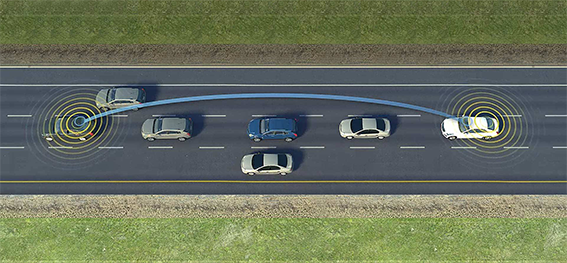
\includegraphics[width=.85\textwidth]{v2v-1d.png} \\
		\vspace{7pt}
		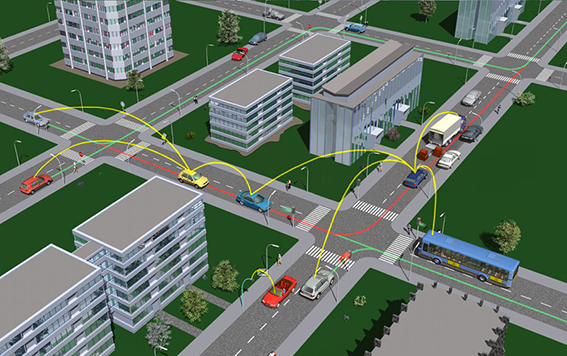
\includegraphics[width=.85\textwidth]{v2v-2d.png}
\caption{Esempio di propagazione di un messaggio in una e due dimensioni (fonti: TheDrive e Car2Car).\label{fig:v2v-1d-2d}}
\end{figure}
%

%!TEX TS-program = xelatex
%!TEX encoding = UTF-8 Unicode
%!TeX spellcheck = it_IT
%!TEX root = ../tesi.tex

\chapter{Modello a ostacoli}\label{chap:modello-a-ostacoli}
%
\section{Il modello matematico}\label{sec:il-modello-matematico}
Il modello utilizzato viene descritto per la prima volta in~\cite{5720204}, dove viene presentato
come un'estensione dei cosiddétti modelli di attenuazione del segnale.
In generale, questi possono essere scritti nella forma dell'Equazione~\ref{eq:fading-models}, dove $P$ è la potenza del trasmettitore (e ricevitore),
$G$ i guadagni delle antenne e $L$ il termine che indica le attenuazioni dovute alla trasmissione.
%
\begin{gather}
	P_r[dBm] = P_t[dBm] + G_t[dB] + G_r[dB] - \sum L_x[dB] 														\label{eq:fading-models} \\
	L_{TwoRayGround} = 10 \lg \left( \frac{d^4 L}{h^2_t h^2_t} \right)	\qquad [dB]		\label{eq:tworayground-model} \\
	L_{LogNorm} = 10 \lg \left( X_\sigma \right)	\qquad [dB]													\label{eq:lognorm-model}
\end{gather}
%
Questi modelli possono essere espressi come componenti di $L$ e concatenati in modo da ottenere l'attenuazione totale risultante.
Ad esempio, le equazioni~\ref{eq:tworayground-model} e~\ref{eq:lognorm-model} illustrano rispettivamente i modelli a doppio raggio e log-normale.

Il modello in esame rappresenta la perdita di segnale dovuta a un ostacolo estendendo l'Equazione~\ref{eq:fading-models}
col termine $L_{s,o}$, che unisce l'attenuazione causata dai bordi dell'ostacolo (attenuazione per-parete)
e quella derivante dalla superficie interna (attenuazione per-metro):
%
\begin{gather}\label{eq:osbtacle-model}
	L_{s,o} = \alpha n + \beta d_o
\end{gather}
dove $n$ è il numero di volte che il bordo dell'ostacolo viene intersecato dalla visuale e $d_o$ è la distanza, in metri, attraversata all'interno dell'ostacolo.
Il primo dei due parametri di calibrazione, $\alpha$, espresso in decibel per metro (dB/m), descrive l'attenuazione
che la trasmissione subisce a causa delle pareti esterne dell'ostacoli.
Il secondo, $\alpha$, espresso in decibel (dB per parete), serve come misura di approssimare della struttura interna dell'ostacolo.
Tramite la regolazione di questo valore è possibile rappresentare diverse tipologie di ostacoli.

Prendendo il caso di edifici in un ambiente cittadino, i valori predefiniti per i due parametri sono $\alpha = 9$ dB per parete e $\beta = 0,4$ dB/m.
%
\begin{figure}[htbp]
	\centering
		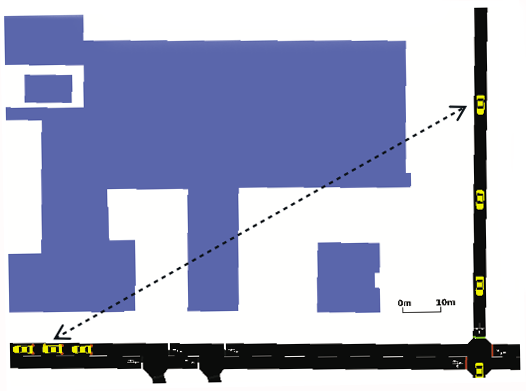
\includegraphics[width=.6\textwidth]{carpenter-1.png}
\caption{Esempio di scenario urbano.\label{fig:scenario-urbano-1}}
\end{figure}
%
Prendiamo l'esempio raffigurato in \figurename~\ref{fig:scenario-urbano-1}, dove la linea fra i due veicoli interseca $n=6$ muri e una distanza interna di $d_o=32$m;
sostituendo i valori in~\ref{eq:osbtacle-model} si ottiene: $L_{s,o} = 9*6 + 0,4*32 = 66,8$dB.
Si evince come, con questa quantità di attenuazione, sia difficile che la trasmissione da un veicolo abbia abbastanza potenza per essere ricevuta dal secondo veicolo.
%
\section{L'implementazione}\label{sec:implementazione}
Ripredendo il modello ideato in~\cite{5720204} e descritto nella sezione precedente, in~\cite{Carpenter:2015:OMI:2756509.2756512} gli autori ne hanno sviluppato
un'efficiente implementazione per il software di simulazioni ns-3, chiamato \textit{Obstacle Shadowing}.
Un ostacolo è rappresento come un poligono bidimensionale, internamente riprodotto da una lista di vertici $(x,y)$; il poligono delimita
il confine (i bordi) dell'ostacolo.
Nel codice inserito in ns-3 sono state utilizzate le Computational Geometry Algorithms Library (CGAL), libreria scritta in \Cpp contente algoritmi di geometria computazionale.
Gli ostacoli sono raggruppati in una struttura algebrica dedicata, chiamata partizione binaria dello spazio (\textit{Binary Search Partition}, BSP), utilizzata
per motivi di ottimizzazione.
% la ricerca dei potenziali ostacoli nella linea di visuale fra due nodi.

Nel dettaglio, quando bisogna calcolare l'attenuazione del segnale fra due nodi, si prende in considerazione un rettangolo fittizio che include i due nodi, lo si estende
di un certo raggio, ad esempio $200$ metri; i potenziali ostacoli si trovano cercando il punto centrale dell'ostacolo all'interno del BSP.
Ogni ostacolo il cui centro si trova all'interno della regione descritta in precedenza viene controllato per verificare se interseca la visuale
(in questo caso \textit{obstructed-line-of-sight}, OLOS), fra i due nodi.
Se questa verifica ha esito positivo (il segnale interseca effettivamente un ostacolo), viene cacolato il numero di intersezioni e la distanza interna percorsa e,
successivamente, restituita la quantità di attenuazione secondo la Formula~\ref{eq:osbtacle-model}.
Questo processo è riassunto nell'Algoritmo~\ref{algo:algoritmo-getobstucteddistancebetween}.
Infine, come ulteriore ottimizzazione, il valore calcolato viene salvato e riutilizzato nel caso i nodi non si siano spostati per più di $0,1$ metro.
%
\begin{italianalgorithm}[h]
\caption{Algoritmo per determinare il numero di intersezioni con i bordi dell'ostacolo e la distanza interna percorsa fra due punti.}\label{algo:algoritmo-getobstucteddistancebetween}
\begin{algorithmic}[1]
	\Procedure{GetObstuctedDistanceBetween}{$p_1, p_2, B$}
	\BState{}\emph{Input}: $p_1, p_2$: posizione dei due veicoli; $B$: partizione binaria dello spazio (BSP) di ostacoli.
	\BState{}\emph{Output}: Distanza interna percorsa, $m_o$, e il numero di intersezioni con i bordi, $n$.
	\State{$m_o \gets 0;\; n \gets 0$}
	\TextState{Inizializza la portata massima $r$: distanza dal punto $p_1$ o $p_2$ al centro di un ostacolo, utilizzata per filtrare il sottoinsieme di ostacoli sufficientemente vicini.}
	\TextState{Crea un riquadro di delimitazione $b$ per $p_1$ e $p_2$ ed estendila di $r$ in tutte le direzioni.}
	\TextState{Calcola l'insieme di potenziali ostacoli $O$ da quelli all'interno di $b$ in $B$.}
	\ForEach{ostacolo $o \in O$}
		\If{(distanza($p_1$, o.centro) $< r$) $\vee$ (distanza($p_2$, o.centro) $< r$)}
			\ForEach{spigolo $e \in o$}\label{algo:line:getobstucteddistancebetween-interesezione}
				\If{$s$ interseca un raggio da $p_1$ a $p_2$}
					\State{$n \gets n+1$}
					\TextState{Salva la distanza minima e massima da $\{ p_1, p_2\}$ al punto d'intersezione.}
				\EndIf{}
				\TextState{$m_o \gets m_o+$ differenza fra i valori min e max calcolati al passo precedente.}
			\EndFor{}
		\EndIf{}
	\EndFor{}
	\Return{$m_o$ e $n$}
	\EndProcedure{}
\end{algorithmic}
\end{italianalgorithm}
%
Per quanto rigurda la struttura del codice in ns-3, il modello è implementato in tre classi:
\textsf{Obstacle} contiente la rappresentazione geometrica dell'ostacolo come anche i parametri dell'attenuazione per-metro e per-muro.
\textsf{Topology} legge il file contente le informazioni sugli ostacoli (vedere capitolo successivo) e per ognuno di questi
lo crea e lo posiziona all'interno della struttura dati BSP.
La terza, \textsf{ObstacleShadowingPropagationLossModel}, estende ns-3 aggiungendo il modello di propagazione a ostacoli
e richiama \textsf{Topology} nel momento in cui si rende necessario calcolare l'attenuazione del segnale fra due nodi,
utilizzando l'Algoritmo~\ref{algo:algoritmo-getobstucteddistancebetween}.
Il tutto è incluso in un nuovo modulo chiamato \textsf{obstacle} (ostacolo).
%
\section{Estensione a tre dimensioni}\label{sec:estensione-a-tre-dimensioni}
Come detto in precedenza, gli oggetti sono rappresentati da poligoni bidimensionali e, conseguentemente,
il modello descritto lavora in una proiezione bidimensionale dell'ambiente (tridimensionale) di ns-3,
prendendo quindi in considerazione solo le prime due componenti \textit{x} e \textit{y} della posizione di ogni nodo.

Uno dei principali motivi che portò gli ideatori del modello a questa scelta fu la mancanza di sufficienti informazioni tridimensionali
sulla piattaforma dalla quale aquisivano i dati (OpenStreetMap, OSM).
Grazie all'avanzamento del progresso tecnologico e a una crescente diffusione di Internet, questi dati
sono, e saranno sempre più, disponibili per un numero crescente di aree.
Dato, quindi, il supporto nativo alla terza dimensone di ns-3 (a differenza dei suoi precedessori) e la crescente diffusione
di dati trimensionali su edifici e ostacoli in generale sulle nostre città, è naturale pensare di estendere il modello affinché
tenga conto di questa componente e pertanto dell'esatta posizione del nodo nell'ambiente della simulazione.
%
\subsection{Altezza degli edifici}\label{subsec:altezza-edifici}
Sebbene le forma degli edifici si possa descrivere esclusivamente in due dimensioni (punti bidimensionali che ne delineano il perimetro al suolo),
OSM prevede la possibilità di definire l'altezza totale in metri e/o specificare il numero di piani (sopra e sotto il livello del suolo)
presenti.
Questa informazione può essere sfruttata per creare una forma tridimensionale semplificata dell'edificio.
%
\begin{figure}[htbp]
	\centering
		\fbox{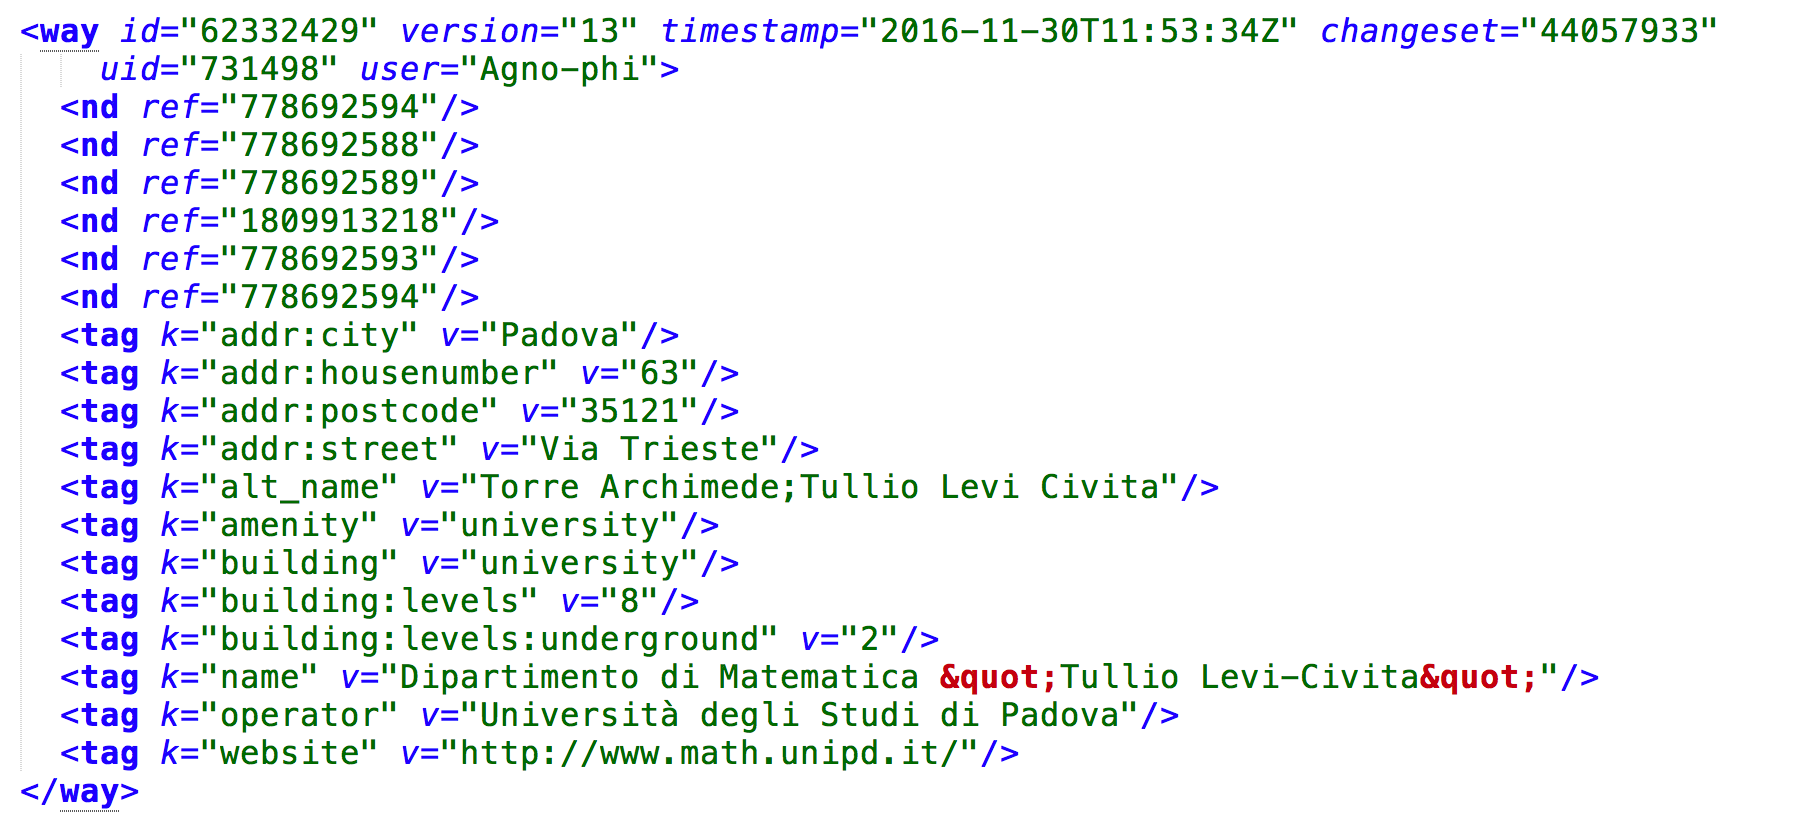
\includegraphics[width=\textwidth]{file-pd-osm-unipd.png}}
\caption{File dati estratto da OSM in cui compaiono informazioni sull'altezza di un edificio.\label{fig:esempio-pd-osm-edificio-altezza}}
\end{figure}
%
Nell'esempio indicato nel \figurename~\ref{fig:esempio-pd-osm-edificio-altezza}, manca la misura dell'altezza ma è presente
il numero di piani: è sufficiente moltiplicare questo numero, qui $8$, per l'altezza media un piano, per esempio $2,7$ metri,
per ottenere una stima dell'altezza pari a $21,6$ metri.
%
\begin{figure}[htbp]
	\centering
	\fbox{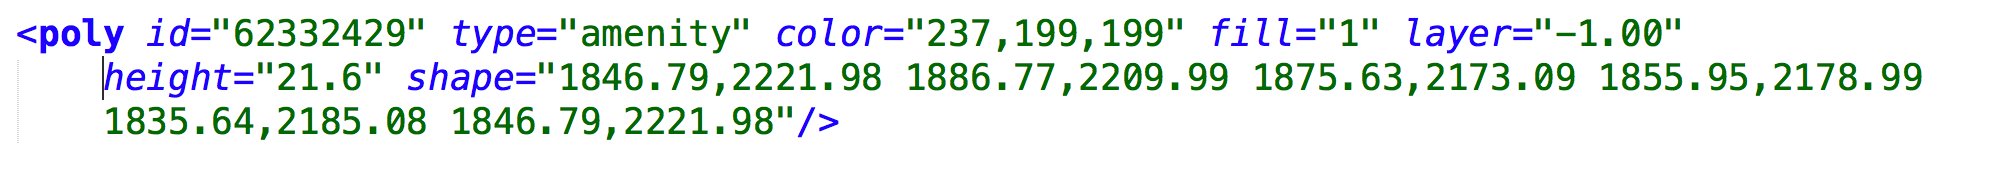
\includegraphics[width=\textwidth]{esempio-poly-blocco-torre.png}}
\caption{Rappresentazione di un edificio in cui è presente un valore di l'altezza.\label{fig:esempio-pd-osm-edificio-altezza}}
\end{figure}
%
\subsection{Modifica dell'algoritmo}\label{subsec:modifica-all-algoritmo}
Il resto dell'algoritmo \textsf{GetObstuctedDistanceBetween} (Algoritmo~\ref{algo:algoritmo-getobstucteddistancebetween})
rimane sostanzialmente lo stesso e, nello specifico, la ricerca dei potenziali ostacoli rimane invariata.
Infatti gli ostacoli che si interpongono fra due punti nello spazio tridimensionale saranno gli stessi che sul piano bidimensionale
(creato dalla perdita della terza componente \textit{z}) in quanto gli ostacoli che vengono considerati sono ``ancorati'' al terreno ($z=0$).
Anche l'oggetto \textsf{Obstacle} rimane quasi del tutto invariato, fatta eccezione per l'aggiunta del valore l'altezza.

Le modifiche significative risiedono quasi totalmente nel calcolo delle intersezioni fra l'ostacolo e il raggio che collega i due nodi.
In origine, l'intersezione veniva calcolata fra il segmento (raggio) che unisce i due punti e lo spigolo dell'ostacolo considerato in quel
momento, procedura poi iterata per ogni spigolo dell'ostacolo (riga~\ref{algo:line:getobstucteddistancebetween-interesezione}).
È possibile, tuttavia, considerare il piano perpendicolare al suolo passante per lo spigolo e trovare l'intersezione fra questo
e il raggio passante per i due punti; il punto risultante (se esiste) sarà allora tridimensionale.
A questo punto si rende necessario però controllare che il punto trovato sia ``valido'', ossia compreso fra il segmento inferiore
(quello considerato al momento), il segmento superiore parallelo a questo di altezza pari a quella dell'ostacolo e i due segmenti
perpendicolari che congiungono le estemità di questi due segmenti.
Per chiarire il concetto, si pensi a un semplice edificio: definita la forma alla base (al suolo) i muri sono perpendicolari
al terreno e, a una certa altezza, si trova il tetto.
Il punto d'intersezione che interessa si trova sulla faccia del muro (in questa semplificazione i muri non hanno spessore);
una volta generato il piano va controllato che il punto sia un punto valido.

L'ultimo passo, non necessario nel caso bidimensionale, consiste nel controllare che il raggio (fra i nodi)
non intersechi la faccia superiore dell'oggetto (il tetto in un edificio); questo viene fatto esattamente come nei passi precedenti.
Le modifiche sono riportate nell'Algoritmo~\ref{algo:algoritmo-getobstucteddistancebetween-modificato}.
%
\begin{italianalgorithm}[!h]
\caption{Modifica all'algoritmo per includere la terza dimensione.}\label{algo:algoritmo-getobstucteddistancebetween-modificato}
\begin{algorithmic}[1]
	\Procedure{GetObstuctedDistanceBetween}{$p_1, p_2, B$}
	\State{\ldots}
	\setcounter{ALG@line}{7}
	\ForEach{ostacolo $o \in O$}
		\If{(distanza($p_1$, o.centro) $< r$) $\vee$ (distanza($p_2$, o.centro) $< r$)}
			\ForEach{spigolo $e \in o$}
				\TextState{Crea un piano $pl$ passante per $e$ e perpendicalare al suolo}
				\If{$pl$ interseca un raggio da $p_1$ a $p_2$ e il punto è valido}
					\State{$n \gets n+1$}
					\TextState{Salva la distanza minima e massima da $\{ p_1, p_2\}$ al punto d'intersezione.}
				\EndIf{}
				\TextState{$m_o \gets m_o+$ differenza fra i valori min e max calcolati al passo precedente.}
			\EndFor{}
			\TextState{Crea un piano $pls$ a partire dalla faccia superiore dell'oggetto}
			\If{$pls$ interseca un raggio da $p_1$ a $p_2$ e il punto è valido}
				\State{$n \gets n+1$}
				\TextState{Aggiorna la distanza minima e massima di conseguenza.}
			\EndIf{}
		\EndIf{}
	\EndFor{}
	\Return{$m_o$ e $n$}
	\EndProcedure{}
\end{algorithmic}
\end{italianalgorithm}
%


%----------------------------------------------------------------------------------------
%	FOOTERS
%----------------------------------------------------------------------------------------

\addcontentsline{toc}{chapter}{References}
\bibliography{../utils/biblio.bib}
\bibliographystyle{ieeetr}

%----------------------------------------------------------------------------------------
%	END
%----------------------------------------------------------------------------------------
\end{document}
